\chapter{Git}\label{cha:Git}
In diesem Kapitel werden auf die wesentlichsten Grundlagen und Befehle
beschrieben, um mit Git Dateien zu verwalten. Als Erstes wird mit einfachen
Befehlen ein Git-Repository erstellt und später am Beispiel dieses Repositorys,
auf weitere Eigenschaften und fortgeschrittene Befehle eingegangen.
Außerdem stellt der Autor dieser Seminararbeit, den Quellcode dieser Arbeit als
Git-Repository unter \cite{link:seminararbeit} zur Verfügung. Dieses Repository
dient ebenso als Beispiel für Sachverhalte, bei denen der gewünschte
Zusammenhang hiermit besser darzustellen ist.

\section{Grundlagen}\label{gitbasics}
In diesem Beispiel werden wir ein Repository \textit{git-example} mit einem
Skript (\texttt{git-stats}) erstellen welches ein paar einfache Statistiken
über die Autoren eines git Repositorys erzeugt.

Alle Beispiele werden auf einer Linux Kommandozeile durchgeführt. Git ist für
alle gängigen Linux Derivate verfügbar. Die Autoren von \cite[S.~12-14]{progit}
gehen auf weitere Details zur Installation von Git in anderen Versionen oder
auf anderen Betriebssystemen ein.

Die in den Beispielen eingesetzte Version von Git ist 2.15.0. Der folgende
Abschnitt basiert zum Zeil auf den Ausführungen der Autoren aus
\cite[S.22-57]{gitops}

\lstinputlisting[
  label=lst:gitversion,
  caption={Version von Git ausgeben},
  captionpos=none,
]{listings/git_version.lst}

\subsection{Konfiguration}\label{gitconfig}
Zu Beginn sollten einige grundlegende Konfigurationen vorgenommen werden. So
sollten, damit die Nachvollziehbarkeit gewährleistet ist als erstes immer der
Name und die Mailadresse des Benutzers konfiguriert werden. Auch ist die
farbliche Darstellung der Ausgaben durchaus hilfreich. Hier kann Git so
konfiguriert werden, dass die Farbausgabe automatisch unterdrückt wird sollte
die Ausgabe in eine Datei umgeleitet werden.

\lstinputlisting[
  label=lst:gitinitconfig,
  caption={Erste Git Konfiguration},
  captionpos=none,
]{listings/git_init_config.lst}

Die \textit{global} eingestellten Optionen können ebenfalls direkt in der Datei
\texttt{\textasciitilde/.gitconfig} eingesehen und bearbeitet werden.
Zusätzlich können für jedes Repository spezifische Konfigurationen vorgenommen
werden. Hierzu muss der Parameter \texttt{--global} bei dem o.a. Befehl
entfernt werden. Die zugehörige Konfigurationsdatei findet sich in jedem
Repository unter dem Pfad \texttt{.git/config}.

\subsection{Erstellen eines Repositorys}\label{startup}
Damit Dateien nun mit Git versioniert werden können, muss wie folgt ein
(lokales) \gls{repository} erstellt werden:

\lstinputlisting[
  label=lst:gitinit,
  caption={Repository anlegen},
  captionpos=none,
]{listings/git_init.lst}

Sollte das Verzeichnis \texttt{hello\_seminar.git} noch nicht existieren, wird
es angelegt. Zusätzlich wird innerhalb von \texttt{hello\_seminar.git} noch ein
weiteres Verzeichnis \texttt{.git} erzeugt, in dem, neben der Konfiguration,
alle Daten abgelegt werden die Git zur weiteren Verwaltung des \glspl{repository}
benötigt.

Um den Status des aktuell erzeugten \glspl{repository} auszugeben kann der
Befehl \texttt{\$ git status} verwendet werden:

\lstinputlisting[
  label=lst:gitstatus,
  caption={Status des Repositorys ausgeben},
  captionpos=none,
]{listings/git_status.lst}

Die von Git erzeugte Ausgabe macht darauf aufmerksam, das noch keine Commits
erzeugt wurden und dass man nun neue Dateien erstellen und hinzufügen kann.

\subsection{Die ersten Commits}\label{sec:first_commits}

Wir werden nun die ersten Dateien zu dem Repository hinzufügen. Dazu laden wir
zwei Dateien mit folgendem Befehl aus dem Internet herunter. Zuvor sollte aber
noch mit folgendem Befehl \texttt{\$ mkdir helpers} ein Unterordner in dem
erzeugten Repository angelegt werden. Wer diese Dateien nicht herunterladen
kann oder möchte, darf selbstverständlich auch einfach Dateien mit gleichem
Namen und beliebigem Inhalt erstellen.

\lstinputlisting[
  label=lst:downloads,
  caption={Herunterladen der Beispieldateien},
  captionpos=none,
]{listings/downloads.lst}

Ab jetzt können die Dateien mit \gls{git} verwaltet werden. Ein erstes
Hinzufügen einer Datei mit dem Befehl \texttt{\$ git add LICENSE} führt zu
folgender Ausgabe von \texttt{\$ git status}:

\lstinputlisting[
  label=lst:add_first_file,
  caption={Eine erste Datei hinzufügen},
  captionpos=none,
]{listings/add_first_file.lst}

Die Ausgabe macht darauf aufmerksam, dass zum Einen, eine neue Datei zum Commit
vorgemerkt ist und zum Anderen, dass sich noch eine Datei im Verzeichnis
befindet, die wir noch nicht mit Git verwalten. Hierbei ist anzumerken, dass
Git auch die vorgemerkte Datei noch nicht wirklich versioniert. Dazu müssen wir
zuerst einen Commit erstellen. Darauf wie Git hier unterscheidet, wird im
Späteren (Abschnitt \ref{sec:trees} auf Seite \pageref{sec:trees}) nochmal
eingegangen.

Der erste Commit in dem angelegten Repository wird mit dem Befehl \texttt{\$
git commit} erzeugt. Eine Bemerkung zu dem Commit kann, je nach
voreingestelltem Systemeditor jetzt eingegeben werden oder optional mit dem
Parameter \texttt{-m} direkt auf der Kommandozeile übergeben(Listing
\ref{lst:git_first_commit}). In der Bemerkung wird die erste Zeile als Betreff,
und getrennt mit einer Leerzeile alle weiteren Zeilen als ausführliche
Beschreibung verwendet. Dieses Format ist, i.d.R. in den meisten
Versionskontrollsystemen üblich.

\lstinputlisting[
  label=lst:git_first_commit,
  caption={Der erste Commit},
  captionpos=none,
]{listings/git_first_commit.lst}

Darüber hinaus bietet es sich an, sich bem Erstellen solcher Bemerkungen an sich
an gewisse Regeln zu halten. Beispielsweise beschreiben Jez Humble und David
Farley in \cite[S.~37]{cd} eine übliche Situation, bei dem es durchaus sinnvoll
kann, nicht nur zu wissen was der Autor geändert hat, sondern auch warum
und in welchem Kontext. Wenn nicht klar ist, was der Autor sich bei
Änderungen gedacht, hat oder Zusammenhänge nicht aus dem Commit hervorgehen, kann
ein gefundener und behobener Fehler vor dem Veröffentlichen einer
Softwareversion durchaus zu Folgefehlern führen. Solche Situationen enden
nicht selten darin, dass viele Stunden Arbeit investiert werden müssen diese zu
bereinigen.\cite[S.~37]{cd}

Nachdem der erste Commit erzeugt wurde, kann dieser nun mit \texttt{\$ git
show} (Abschnitt \ref{sec:gitshow} auf Seite \pageref{sec:git_show}) betrachtet
werden. In diesem Fall wurde beispielhaft eine etwas ausführlichere Bemerkung
gewählt:

\lstinputlisting[
  label=lst:git_show_first_commit.lst,
  caption={Anzeige des ersten Commits},
  captionpos=none,
]{listings/git_show_first_commit.lst}

Hier können alle wichtigen Informationen eingesehen werden. Neben Zeitpunkt,
Autor und Beschreibung auch die \textit{Commit-ID} (Abschnitt \ref{sec:commit}
auf Seite \pageref{sec:commit}). Die weiteren Informationen werden in einem
Format namens Unified-Diff dargestellt, auf welches hier nicht weiter
eingegangen wird. Details zu dem Format stellen die Autoren von \textit{GNU
diffutils} unter \cite[S.~12-13]{paper:diffutils} zur Verfügung.

Wir fügen nun die zweite Datei mit einem weiteren \texttt{\$ git add} hinzu:

\lstinputlisting[
  label=lst:git_add_second_file,
  caption={Eine weitere Datei hinzufügen},
  captionpos=none,
]{listings/git_add_second_file.lst}

Anschließend erzeugen wir einen weiteren \gls{commit} mit:

\lstinputlisting[
  label=lst:commit_git-stats,
  caption={Hinzufügen einer weiteren Datei},
]{listings/commit_git-stats.lst}

Mit diesen beiden zuvor ausgeführten Commits haben wir nun eine, wenn auch
kurze, Historie erstellt. Um diese zu untersuchen dienen die Befehle \texttt{\$
git whatchanged}\footnote{Der Befehl \texttt{\$ git whatchanged} stammt aus
frühen von Git und ist das gleiche wie \texttt{\$ git log} mit einigen
Parametern um die Ausgabe entsprechend zu Formatieren.} oder \texttt{\$ git
log}. Wir werden in Abschnitt \ref{sec:gitlog} weiter darauf eingehen aber für
diesen Fall ist \texttt{\$ git whatchanged} ausreichend:

\lstinputlisting[
  label=lst:first_git_whatchanged.lst,
  caption={Untersuchen der Historie},
  captionpos=none,
]{listings/first_git_whatchanged.lst}

Die Ausgabe wird im sogenannten \textit{raw} Format dargestellt. Es werden alle
Commits mit Informationen über den Autor, Commit-ID, Zeit und den veränderten
Dateien in zeitlicher Reihenfolge dargestellt. Die konkreten Veränderungen am
Inhalt der Dateien werden hier nicht dargestellt(Abschnitt \ref{sec:gitlog} auf
Seite \pageref{sec:gitlog}).

Erwähnenswert ist noch das Git, im Gegensatz zu anderen
Versionskontrollsystemen, die Dateiberechtigungen speichert. Wer bei den
letzten der beiden Commits auf die Ausgabe geachtet hat (Listing
\ref{lst:commit_git-stats} auf Seite \pageref{lst:commit_git-stats}) dem ist
vielleicht folgende Zeile aufgefallen:

\lstinputlisting[
  label=lst:create_mode,
  caption={Create Mode},
  captionpos=none,
]{listings/create_mode.lst}

Diese Ausgabe besagt das es sich hierbei um eine normale Datei handelt (100)
die mit einer, unter Unix üblichen, Berechtigung (664) angelegt ist. Damit
diese Datei aber entsprechend ausführbar ist, müssen wir noch einen weiteren
Commit, mit einer Änderung an den Dateiberechtigungen, erzeugen:

\lstinputlisting[
  label=lst:git_commit_all,
  caption={Commit mit allen Änderungen},
  captionpos=none,
]{listings/git_commit_all.lst}

Mit dem zuvor ausgeführten Befehl haben wir einen Commit erzeugt ohne unsere
Änderungen vorher mit \texttt{\$ git add} hinzuzufügen. Der Parameter
\texttt{-a} bewirkt hier das alle vorhandenen Änderungen zu einem Commit
zusammengefasst werden und nicht einzeln hinzugefügt werden müssen. Zu beachten
ist allerdings das Dateien die Git noch nicht kennt, davon nicht betroffen
sind. Diese müssen nach wie vor zuerst mit einem \texttt{\$git add} hinzugefügt
werden.

Abschließend zu diesem Abschnitt versehen wir den letzten Commit noch mit einer
Markierung bzw. \gls{tag}.

\lstinputlisting[
  label=lst:git_first_tag,
  caption={Anlegen eines Tags},
  captionpos=none,
]{listings/git_first_tag.lst}

Hiermit haben wir einen \gls{tag} mit dem Namen \texttt{tags/0.0.1} angelegt,
der den letzten Commit (\gls{HEAD}) referenziert:

\lstinputlisting[
  label=lst:git_list_first_tag,
  caption={Listen eines Tags},
  captionpos=none,
]{listings/git_list_first_tag.lst}

Auf den weiteren Umgang mit Tags und welche Arten es gibt wird in den
Abschnitten \ref{sec:tag} und \ref{sec:tagobject} weiter eingegangen.

\subsection{Bäume}\label{sec:trees}
Git organisiert das Repository in drei verschiedene Bereiche. Scott Chacon,
einer der Autoren von \cite{progit}, spricht in einem seiner
Vorträge\cite{link:talesoftrees} von drei Bäumen \textit{HEAD}, \textit{Index}
und dem \textit{Work Tree}.

Den \textit{Work Tree} (Abschnitt \ref{sec:workingtree} auf Seite
\pageref{sec:workingtree}) haben wir bereits als Arbeitsbereich angesprochen.
Mit \gls{HEAD} ist neben dem Verweis auf den neuesten commit auch i.w.S. das
Repository gemeint.  Das Repository(Abschnitt \ref{repository} auf Seite
\pageref{repository}) dient i.d.S. als Datenspeicher für alle Commits, deren
Inhalte und Historie. Der Index(Abschnitt \ref{sec:index} auf Seite
\pageref{sec:index}) in Git stellt, im Vergleich zu voherigen
Versionskontrollsystemen, eine Neuerung dar. Der Index stellt einen Bereich
zwischen dem \gls{repository} und dem Arbeitsbereich dar. Er dient dazu um den
nächsten \gls{HEAD} bzw. Commit vorzubereiten. Die Kommandos \texttt{\$git
add}, \texttt{\$ git reset} und \texttt{\$git commit} arbeiten auf diesen drei
Bereichen.\cite[34-35]{gitosp}

\begin{figure}[h]
    \centering
    \includegraphics[scale=0.60]{images/trees.eps}
    \caption{\textit{Work Tree}, \textit{HEAD} und Index\cite[34]{gitosp}}
    \label{fig:trees}
\end{figure}

\subsection{Objektmodell}\label{sec:objectmodel}
Wie in vorherigen Abschnitten bereits erwähnt, ist das Repository ein
Datenspeicher vergleichbar mit einer Datenbank. Dahinter steht ein Datenmodell
welches sicherstellt, dass die einzelnen Teile eines Commits und deren
Zusammenhänge über die Zeit gewährleistet sind. Dazu verwendet Git ein auf
Objekten basierendes Modell. Dieser Abschnitt geht auf die verschiedenen
Objekttypen und deren Zusammenhänge ein. Er basiert größtenteils auf den
Ausführungen der Autoren aus \cite[S.~49-59]{gitosp}.

Für jedes Objekt wird innerhalb des Repositorys unter \texttt{.git/objects}
eine Datei abgelegt. Für alle Objekte wird eine eindeutige \gls{SHA-1}
Prüfsumme erzeugt, die gleichzeitig als Dateiname und Referenz für das
abgespeicherte Objekt dient. Git unterscheidet zwischen den Objekttypen Tree,
Object, Commit und Tag.

\subsubsection{Trees und Blobs}\label{sec:treeblobobjects}
Zum Speichern von Verzeichnissen verwendet Git ein sogenanntes
\textit{Tree-Object}. Eine Ausgabe der Dateistruktur aus dem verwendeten
Beispiel (Abschnitt \ref{sec:first_commits} auf Seite
\pageref{sec:first_commits}) erhält man mit dem Linux Befehl \texttt{\$ tree}:

\lstinputlisting[
  label=lst:tree.lst,
  caption={Dateibaum des Beispiels},
  captionpos=none,
]{listings/tree.lst}

Um nun den Dateibaum mit der Objektstruktur aus dem Git Repository zur
vergleichen, kann der Befehl \texttt{\$ git ls-tree HEAD} genutzt werden:

\lstinputlisting[
  label=lst:git_ls_tree.lst,
  caption={Objektbaum des Beispiels},
  captionpos=none,
]{listings/git_ls_tree.lst}

Git unterscheidet hier zwischen den angelegten Verzeichnissen und den
eigentlichen Dateien, wie \texttt{helpers/git-stats}. Verzeichnisse werden als
\textit{tree} dargestellt und enhalten, wie auch im Dateisystem, Referenzen auf
weitere Objekte entweder vom Typ \textit{tree} oder \textit{blob}.  Inhalte von
Dateien werden in \textit{blob}-Objekten gespeichert. Allerdings ist der
Dateiname nicht Bestandteil des \textit{blob}, sondern wird in dem
referenzierenden \textit{tree} gespeichert. Dies wird auch nochmal deutlicher,
wenn wir uns das \textit{tree} Objekt zu dem Ordner \texttt{helpers} anschauen:

\lstinputlisting[
  label=lst:git_ls_tree_helpers.lst,
  caption={Objekt eines Ordners},
  captionpos=none,
]{listings/git_ls_tree_helpers.lst}

\begin{figure}[h]
  \centering
  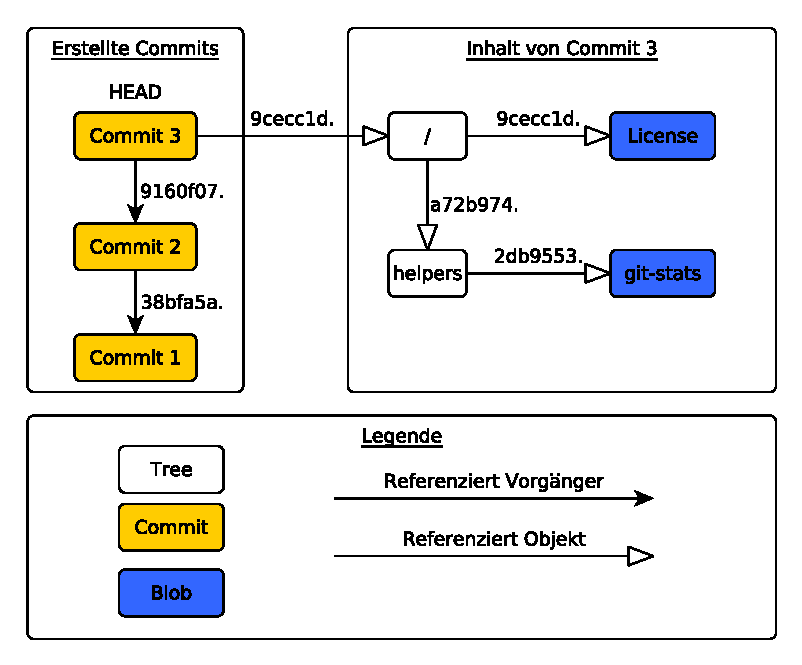
\includegraphics[scale=0.75]{images/objectmodel.eps}
  \caption{Objektmodell zum Beispiel aus Abschnitt \ref{sec:first_commits}\cite[S.~53]{gitosp}}
  \label{fig:objectmodel}
\end{figure}

\subsubsection{Commit}\label{sec:commitobject}
Ein Commit-Objekt enthält, neben den bereits bekannten Daten aus Listing
\ref{lst:git_show_first_commit.lst} eine Referenz zu \textbf{einem}
\textit{tree} und ggf. einem vorhergehenden Commit (engl.  \textit{parent}). Im Fall
eines Merge-Commits (Abbildung \ref{fig:merge} auf Seite \pageref{fig:merge})
werden enstprechend so viele Vorgänger referenziert wie branches
zusammengeführt wurden. Hier wird jeweils auf \gls{HEAD} des jeweiligen
Branches referenziert. Der in einem Commit referenzierte \textit{tree} ist,
immer ein Verweis auf einen sogenannten \textit{top-level-tree} (\texttt{/}).
Dieser Verweis referenziert die Wurzel des entstandenen Objektbaums und enhält
keinen Dateinamen(Abbildung \ref{fig:objectmodel} auf Seite \pageref{fig:objectmodel}).

Dadurch das Jeder Commit seinen vorhergehenden Commit referenziert entsteht ein
gerichteter azyklicher Graph bei dem ein Koten durch einen Commit und Kanten
durch Referenzen repräsentiert werden.\cite[57]{gitops}.

\lstinputlisting[
  label=lst:git_show_raw,
  caption={Ausgabe eines Commits im \textit{raw} Format},
]{listings/git_show_raw.lst}

Zusätzlich unterscheidet Git noch den Committer vom Autor. Diese können sich
unterscheiden wenn Commits z.B. einen Reviewprozess durchlaufen müssen und
nicht von dem Autor selbst in das aktuelle Repository integiert werden(Listing
\ref{lst:git_show_raw}).

\subsubsection{Tag}\label{sec:tagobject}
Ein \gls{tag} markiert einzelne Commits. Hierzu werden i.d.R. Versionsnummern
als Namen verwendet (Abschnitt \ref{sec:tag} auf Seite \ref{sec:tag}). Neben
der \textit{SHA-1-ID} des zu referenzierenden Commits, wird ein Tagname, der
Typ und der Autor (\textit{tagger}) mit Name und Mailadresse gespeichert. Je
nach Art des Tags kann optional noch eine Beschreibung angegeben werden. Bei
Tags ist nicht nur die Prüfsumme, sondern auch der Name eindeutig. Wird
versucht ein Tag mit einem bereits existierenden Namen zu erzeugen, dann
reagiert Git mit einer Fehlermeldung und lehnt das Erstellen entsprechend ab.

Git unterscheidet zwischen drei Arten von Tags:

\begin{enumerate}
\item \textbf{Lightweight Tags:} Dieser Typ ist die einfachste Variante. Er
enthält neben den benötigten Daten wie Autor, Commitreferenz und Prüfsumme
lediglich den Namen. Erzeugt wird er mit dem Befehl:

\lstinputlisting[
  label=lst:git_light_tags,
  caption={Lightweight Tags},
  captionpos=none,
]{listings/git_light_tags.lst}

\item \textbf{Annotated Tags:} Annotated bedeutet nichts Anderes als
kommentiert. Zusätzlich zu den Daten aus den einfachen Tags, wird hier wie bei
einem Commit ein Texteditor geöffnet. Alternativ kann auf der Kommandozeile
ebenfalls mit dem Parameter \texttt{-m} eine Beschreibung übergeben
werden.

\lstinputlisting[
  label=lst:git_annotated_tags,
  caption={Annotated Tags},
  captionpos=none,
]{listings/git_annotated_tags.lst}

\item \textbf{Signierte Tags:} Vorausetzung für diese Art von Tags, ist ein
vorhandener privater \textit{GPG-Key}. Diese Tags werden mit einer Signatur,
versehen die von anderen entsprechend überprüft werden kann, um die Identität
des Autors eindeutig zu verifizieren\footnote{\url{https://gnupg.org}}.
Erstellt werden signierte Tags mit dem zusätzlichen Parameter
\texttt{-s} angelegt:

\lstinputlisting[
  label=lst:git_signatured_tags,
  caption={Signierte Tags},
  captionpos=none,
]{listings/git_signatured_tags.lst}

Zuvor muss Git der zu verwendene Key noch bekannt gemacht werden. Das
kann mit folgendem Befehl erreicht werden:

\lstinputlisting[
  label=lst:git_add_key,
  caption={Signierte Tags},
  captionpos=none,
]{listings/git_add_key.lst}
\end{enumerate}

\subsubsection{Branch}\label{sec:branchobject}
Eine einfache Antwort auf die Frage warum ein Branch nun kein Objekt ist, liefert
das Ausgeben der Referenzdatei des Branches \textit{master}:

\lstinputlisting[
  label=lst:cat_master.lst,
  caption={Referenz \textit{master}},
  captionpos=none,
]{listings/cat_master.lst}

Die ausgegebene Prüfsumme ist in diesem Fall lediglich die \textit{SHA-1-ID} des
letzten Commits aus Abschnitt \ref{sec:first_commits}. Branches sind einfach
Textdateien, die eine Commit-ID zu einem referenzierenden Commit enthalten. Da
diese Referenz veränderbar ist und keine weiteren Informationen enthält, wird
hier kein weiterer Objekttyp benötigt. Da der Name des Branches direkt abhängig
von der erstellten Referenzdatei ist, sind auch die Namen von Branches
eindeutig.

Neben der fortgeschrittenen Manipulation von Git Objekten stellen die Autoren
Scott Chacon und Ben Straub in \cite[S.~408-418]{progit} eine ausführlichere
Sicht auf die Objektverwaltung dar.

\subsection{Kommandos}\label{sec:commands}
Einige der in der Arbeit verwendeten Kommandos werden in diesem Abschnitt
nochmal erwähnt und ggf. um weitere Parameter ergänzt. Aufgrund der begrenzten
Länge dieser Arbeit kann an dieser Stelle weder auf alle Git Kommandos noch auf
alle Parameter eingegangen werden. Die verwendeten Kommandos werden aber um
einige wenige Kommandos ergänzt die für die alltägliche Arbeit mit Git sinnvoll
sind.

Alle Git Kommandos bieten eine Vielzahl an Optionen. Eine Übersicht über die
unterstützten Optionen kann mit den unter Linux üblichen Methoden angezeigt
werden. So z.B. mit \texttt{\$ git <Befehl> help} oder mit dem klassischen
Aufruf der Manpage \texttt{\$ man git <Befehl>}.

Viele der Kommandos erwarten ein bestimmtes Argument auf dem sie Arbeiten. So
findet man häufig Argumente die als \textit{tree-ish} oder \textit{commit-ish}
bezeichnet werden. Damit sind aber lediglich entsprechende Objekte gemeint die
z.B. einen Tree referenzieren.\cite[52]{gitosp} So benötigt \texttt{\$ git
ls-tree} aus Abschnitt \ref{sec:objectmodel} ein \textit{tree-ish} und
\texttt{\$ git show} kann auf allen Objecten aus Abschnitt
\ref{sec:objectmodel} arbeiten.

\subsubsection{git add}\label{sec:gitadd}
Mit \texttt{\$ git add} können grundsätzlich Dateien hinzugefügt werden. Der
Befehl selbst bietet, wie fast alle Git Kommandos eine Vielzahl an Optionen.
Eine sei an dieser Stelle besonders erwähnt, \texttt{\$ git add -p}. Das
\texttt{-p} ermöglicht, die durchgeführten Änderungen an den Dateien selektiv
hinzuzufügen. Das kann hilfreich sein, um Änderungen an verschiedenen Teilen in
einzelne \glspl{commit} aufzuteilen oder bestimmte Änderungen wegzulassen.

\subsubsection{git rm}
\subsubsection{git clone}
\subsubsection{git push}
\subsubsection{git log}\label{sec:gitlog}
\subsubsection{git show}\label{sec:gitshow}
Git show gibt alle relevanten Informationen eines Commits aus.....S.25 gitosp
\subsubsection{git tag}
\subsubsection{git branch}
\subsubsection{git mv}

\section{Workflows}\label{sec:Workflows}
\section{Fortgeschrittene Konzepte}
\label{sec:FortgeschritteneKonzepte}
\subsection{Regressionen und Bisektion}\label{sec:bisec}
\subsection{Rebase}\label{sec:rebase}
\subsection{Andere Versionsverwaltungssysteme und Git}
\label{sec:AndereVersionsverwaltungssystemeundGit}
